\chapter{Data Acquisition and Software}
\label{chap:\currfilebase}


\section{Data acquistion}

The \ac{DAC} system developed in this thesis is an open source Arduino based system consisting of multiple microcontrollers. All signal channels are transmitted to a central microcontroller before passing it to a computer that serves as visualization and analysis tool.

\begin{figure}[!htb]
    \centering
    \subcaptionbox{Without signal conditioning\label{sfig:dac_comp_simple}}
        {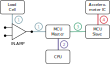
\includegraphics[scale=0.5]{\imgpath/dac/dac_components/dac_comp_simple}}
        \hfill
    \subcaptionbox{With signal conditioning and external \ac{ADC}\label{sfig:dac_comp_precond}}
        {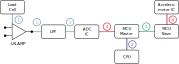
\includegraphics[scale=0.5]{\imgpath/dac/dac_components/dac_comp_precond}}
    \\[0.5em]
    \caption[DAC building blocks]{\acs{DAC}-system building blocks}
    \label{fig:dac_building_blocks}
\end{figure}

\begin{table}[!htb]
    \centering
    \def\linelabel#1#2{%
        \begin{tikzpicture}[%
            x=1em,y=1ex,
            baseline=(N.south),
            font={\fontsize{6pt}{6.2pt}\selectfont},
            ]%
            \draw[#1, line width=1pt] (0,1) -- (1,1) node [
                midway, above, yshift=1,
                circle, fill=white, draw=#1, line width=1pt,
                inner sep=2pt, minimum size=8pt, align=center,
                ] (N) {#2};
        \end{tikzpicture}
    }
    \footnotesize
		\begin{tabular}{c@{ :\hskip 0.5em}l}
            \toprule
            \multicolumn{2}{c}{Interfaces}\\
            \midrule
            \linelabel{WesMixL8qual0}{1} & Analog Signal\\
            \linelabel{WesMixL8qual3}{2} & \ac{USB}\\
            \linelabel{WesMixL8qual4}{3} & \ac{RS}-485\\
            \linelabel{WesMixL8qual6}{4} & \ac{SPI}\\
			\bottomrule
		\end{tabular}
    \normalsize
    \caption[Legend to DAC building blocks]{Legend to \figref{fig:dac_building_blocks}}
\end{table}

\subsection{Building Blocks}

Building blocks are the main components used in the \ac{DAC} signal chain. Additional components that are required to enable the stable operation of the building blocks are not listed.

Because the of accelerometer \ac{IC} output interfaces it is not possible to connect all sensors directly to one \ac{MCU} that acts as a \ac{DAC}. We need to transform the signal to a different interface. A low-cost and versatile method to achieve this is to use a \ac{MCU} for each accelerometer \ac{IC}. These read read the sensor \ac{IC} registers and communicates to the \ac{MCU} master. The master on the other hand acts as a passthrough and transmits the data to the \ac{CPU}. In the setup used it also reads out the \ac{LC} signal. \tabref{tab:mcu_used} lists the \ac{MCU}s used during this thesis. Other components can be found in \autoref{apx:appendix}.

The analog signal output of the \ac{LC} needs to be amplified to match the input range of the \ac{ADC}. To gain the maximum resolution this depends on the expected input range. To get a higher value resolution than offered by the \ac{MCU} embedded \ac{ADC} one can set in an external \ac{ADC} \ac{IC} upstream to the \ac{MCU}. Additionally, we use a \ac{LPF} in \figref{sfig:dac_comp_precond}. The \ac{LPF} is needed to cut off high frequency components of the signal that occur particularly in sharp impulse signals. This design choice may lead to problems because it is not standard procedure, when developing a measurement instrument. Typically components in the analog signal chain are chosen based on the frequency bandwidth of the input signal. This means the cut-off frequency of the \ac{LPF} is set above the signal bandwidth. But because we use low-cost components in our system, the bandwidth is limited to half the sampling rate of the slowest sensor. According to the Nyquist frequency theorem, the cut-off frequency then needs to be reduced to half the sampling frequency potentially reducing the output magnitude of higher frequency components of the signal.

\begin{table}[!htb]
    \centering
    \def\coltitle#1{\multicolumn{1}{c}{#1}}
    {\renewcommand{\arraystretch}{2.5}%
    \footnotesize
		\begin{tabular}{lcccccc}
            \toprule
            \coltitle{Name} &
            \coltitle{Core} &
            \coltitle{\makecell{\ac{ADC}-Reso-\\lution / \si{bit}}} &
            \coltitle{\makecell{Operating\\Voltage / \si{\volt}}} &
            \coltitle{\makecell{Clock Speed\\ / \si{\mega\hertz}}} &
            \coltitle{\makecell{Flash Me-\\mory / \si{\kilo Byte}}} &
            \coltitle{\makecell{SRAM\\ / \si{\kilo Byte}}}\\
            \midrule
            Arduino Due & \makecell{AT91SAM3\\ARM Cortex} & 12 & 3.3 & 84 & 512 & 96\\
            Teensy 3.2 & \makecell{MK20DX256VLH\\Cortex-M4} & \makecell{13\\ \scriptsize{(\SI{16}{bit}-values)}} & 3.3 & 72 & 256 & 64\\
            \makecell[l]{Robotdyn\\Blackpill} & \makecell{STM32F103C8\\Cortex-M3} & 12 & 72 & 64 & 20\\
            \bottomrule
		\end{tabular}
    \normalsize
    }
    \caption[MCUs used]{List of \ac{MCU}s used in this work}
    \label{tab:mcu_used}
\end{table}


\subsection{Interfaces}

The interfaces are the connections and protocols between the different building blocks of the \ac{DAC} system. The interfaces are chosen based on the sensors used, and the expected data rate at the required cable length between each section. I.e.:

\begin{itemize}
    \item Between the analog \ac{LC} and the external \ac{ADC} in \figref{sfig:dac_comp_precond} and the \ac{MCU} integrated \ac{ADC}  in \figref{sfig:dac_comp_simple} respectively the signal transmission is analog.
    \item The register of the accelerometer \ac{IC} is accessed via \ac{SPI}
    \item The communication between \acs{MCU}s is rooted in \acs{RS}-485 differential transmission to accommodate for signal transmission over cable lengths greater than \SI{10}{\meter} and uses a specialized protocol to keep data packages as small as possible.
    \item Between the \ac{MCU} and the \ac{CPU} \ac{USB} transmitts data using the serial class of the Arduino software.
\end{itemize}

Data rates and package sizes are critical when sampling at high frequencies. 

With \ac{RS}-485 data can be transmitted over distances of no less than \SI{100}{\km} at a data rate of \SI{1}{\kilo bit\per\second}. At \SI{1200}{\meter} cable length we can reach data rates of around \SI{100}{\kilo bit\per\second}. In our range of application, i.e. a few tens of \si{\meter}, we can expect data rates of \SI{1}{\mega bit\per\second}. Thus representing the bottle neck in the digital data chain. If we then transmit \SI{80}{bit} bit acceleration measurements (see \figref{fig:data_flow}) at \SI{1.6}{\kilo\hertz} we stay below this expected limit by a safety factor of more than 10.
In arduino the serial package parses all data as in the human readable \ac{ASCII} code. In this format every digit of the integer values are passed as \SI{8}{bit} value. Which means that the a \SI{32}{bit} timestamp and a single axis acceleration are passed as 10\SI{8}{bit}-values and 6\SI{8}{bit}-values respectively. This increases the size of an accelerometer package to \SI{624}{bit}, which in turn reduces the safety factor to approximately 1.
It is clear that one cannot use human readable code to transmit the data and guarantee stability at the required sampling rate.


\subsubsection{MCU communication protocol}

The communication protocol for \ac{MCU} to \ac{MCU} and \ac{MCU} to computer was developed for this project.

\begin{table}[!htb]
    \centering
    \includestandalone[scale=1]{\imgpath/software/mcu_com_protocol/mcu_com_protocol}
    \\[0.5em]
    \footnotesize
		\begin{tabular}{c@{ :\hskip 0.5em}l}
			\toprule
            \large{\textcolor{WesMixL8qual6}{<[}/\textcolor{WesMixL8qual6}{]>}} & Start-/End-bytes, represented as \ac{ASCII}\\
            \textcolor{WesMixL8qual0}{\large (reg)} & Registry/Address of the transmission\\
            \textcolor{WesMixL8qual4}{\large (\#Bytes)} & Number of bytes in transmission\\
            \textcolor{WesMixL8qual5}{\large (data)} & Data to transmit\\
			\bottomrule
		\end{tabular}
	\normalsize
    \caption[MCU communication protocol]{Protocol used to communicate between two MCU's and between MCU and computer}
    \label{tab:mcu_com_protocol}
\end{table}

%     output signal that must be amplified by an \ac{IN-AMP} to scale up the signal to the operating range of the consecutive components.

% . to of smart sensor IC are predetermined. With \ac{SPI}Standard interfaces, determined by senor ic
% MCU com based uart length -> differential transmission using the rs-485 protocol, introduces slave master com, only one slave can speak at a time



\subsection{Dataflow}

All \acs{MCU}s operate sequentially.
The dataflow in \ac{MCU} must be sequential. For this reason during a measurement all data is passed to a central \ac{MCU} where it is streamlined to the pc. The central \ac{MCU} or master cycles through all connected \ac{MCU} performing a data request, hold and receive action. As soon as a slave \ac{MCU} gets a request, it transmits a data package from its buffer. The master now receiving the data package will throughput the signal to the \ac{CPU}, where it is stored. By the end of this process the master will jump to the next slave.

All measurements that consist of a \SI{32}{bit}-Timestamp and the measured values pushed into a \ac{FIFO} buffer using the memory of the \ac{MCU} connected to the sensor. Bundled data packages are then translated to the transmission code as defined in \tabref{tab:mcu_com_protocol} and pulled from the buffer. In \figref{fig:data_flow} the data flow is represented of a system that is using only one slave \ac{MCU}, displayed in violet.

Measurements are packaged due to the time the master requires to change the communication to another slave. During these switches no data is transmitted eventually bottlenecking the data rate of the system.

\begin{figure}[!htb]
    \centering
    \includestandalone[width=0.8\linewidth]{\imgpath/software/data_flow/data_flow}
    \caption[Data flow]{Data flow between two MCU's and the CPU}
    \label{fig:data_flow}
\end{figure}

\section{Software}

The software developed during this project is split into the Arduino software running on the \acs{MCU}s and a python based tool to receive and visualize the data via \ac{USB}.

For the instrument to work, some functions are required, while others desired functions are tools that simplify the workflow during measurements and facilitate bug fixes of the software.

The requirements to the software tools are:
\begin{enumerate}[label=\emph{m\arabic*}, itemindent=3em, labelsep=2em]
    \item Read out accelerometer and \ac{LC} data at the maximum sample speed of the accelerometer \ac{IC}. \label{req:read_out}
    \item Synchronize measurements timestamps\label{req:sync}
    \item Initialize measurement by hammer impulse\label{req:init}
\end{enumerate}

The desired software tools are:
\begin{enumerate}[label=\emph{w\arabic*}, itemindent=3em, labelsep=2em]
    \item Continuous real time output of measurement data\label{des:cont_out}
    \item Cache clearing\label{des:cache}
\end{enumerate}

% \subsubsection*{\ref{req:read_out}:}
% The target is to read out data from two or more accelerometer \acs{IC}s and the data from the \ac{LC} in form of the data flow as in \figref{fig:data_flow}.

% values in a \ac{DAC} system with multiple 